\chapter{Federation/Single-Sign on}

Werden mehrere Webapplikationen betrieben, entsteht schnell der Wunsch, Benutzerkonten zwischen diesen Applikationen zu synchronisieren. Die Grundidee ist es, ein unified Authentication/Authorization-Konzept über mehrere Server hinweg zu implementieren. Potentielle Gründe für den Einsatz einer Single-Sign On oder Federation Lösung sind:

\begin{itemize}
	\item SSO erlaubt es mehreren Applikationen eine gemeinsame Login/Logout-Lösung zu verwenden. Dadurch können redundante Lösungen eingespart und duplizierte Sicherheitsprobleme vermieden werden. Nachteil: der Login-Server ist ein Single-Point-of-Failure.
	\item Das gesamte Passwort-Management kann aus der Webapplikation ausgelagert werden. Es müssen keine Passwörter mehr selbst erhoben, bearbeitet oder gespeichert werden.
	\item Die User-Experience ist angeblich besser. Der Aufwand für einen Benutzer einen neuen Account anzulegen wird minimiert.
	\item Durch den Login-Server können weitere Authenticationsservices implementiert worden sein, z. B. Ausweiskontrolle oder eine Multi-Faktor-Authentication.
\end{itemize}

\section{Festival-Beispiel}

Eine gute Analogie ist ein Musikfestival bei welchem Besucher auf dem Festivalgelände Getränke erwerben können. Je nach Alter darf ein Kunde alkoholische oder nicht-alkoholische Getränke kaufen. Müsste nun jeder Getränkestand bei jeder Bestellung Eintrittskarte und den Ausweis (Altersnachweis) des Besuchers kontrollieren, würde dies zu starken Verzögerungen führen.

Um die Situation zu verbessern, werden beim Festivaleingang die Besucher einmalig bei einem Registrationszelt kontrolliert. Jeder Besucher erhält ein Armband um zu beweisen, dass er eine Eintrittskarte besass. In Abhängigkeit vom Alter bekommen Minderjährige Besucher ein blaues Armband, erwachsene Besucher ein rotes Armband. Anhand dieses Armbands (Token) können nun die Getränkestände schnell kontrollieren, ob ein Gast alkoholische Getränke konsumieren darf. Zusätzlich wird über den Besitz des Bands überprüft, ob ein Besucher eine Eintrittskarte besass. Falls ein Besucher bei einem Getränkeshop ohne Band ein Getränk kaufen will, wird er zu dem Registrationszelt  verwiesen.

In diesem Beispiel ist das Registrationszelt der Identity Provider, die Getränkehändler sind Service Provider, das Armband ein Token und der Besucher der Client.

Das Beispiel zeigt auch zwei Probleme von token-basierten Lösungen. Das Armband gilt für die gesamte Dauer des Festivals (im Folgejahr werden andere Farben verwendet). Es gibt keine Möglichkeit einen Teil der Armbänder nach dem ersten Festivaltag zu invalidieren. Ebenso wird klar, dass jegliche Form von Zugriffskontrolle durch das Armband ersetzt wird. Wollen z. B. ein Vater und Sohn beide Alkohol kaufen, kann der Vater initial den Identitätscheck durchführen und dann sein Armband an seinen Sohn weitergeben. Der Vater geht danach wiederholt zum Registrationszelt und kauft sich ein zweites Zugangsband. Mit dem ersten Band kann nun der Sohn beliebig Alkohol kaufen ohne dass auffällt, dass sein Alter dies eigentlich verbieten sollte. Der alleinige Zeitpunkt der Überprüfung (Authorization) geschieht während der Bandausgabe.

\section{OAuth2}

OAuth (Open Authorization) erlaubt es einem Benutzer (Resource Owner) einer Applikation (Client) Zugriff auf Resourcen/Operationen auf einem Server (Resource Server) zu erteilen. Ein Authorization Server wird verwendet um ein Zugriffs-Token für einen definierten Bereich (scope) am Resourcen-Server auszustellen. Zusätzlich zu dem Zugriffs-Token wird zumeist auch ein Refresh-Token ausgestellt mit dem ein Client ein neues Zugriffstoken ohne Benutzerinteraktion generieren kann.

Da die Rechte eines ausgestellten Token im Normalfall nur während der Ausstellung überprüft werden und danach für die gesamte Lebenszeit des Tokens gültig sind, wird bestenfalls eine sehr kurze Lebenszeit im Minutenbereich gewählt. Läuft das Token ab, kann mit den Refresh-Token ein neues Access-Token angefordert werden. Da hierfür keine Benutzerinteraktion benötigt wird, kann dies automatisiert und transparent für den Endbenutzer erfolgen. Der Vorteil liegt darin, dass während der Ausstellung durch den Authorisationsserver die angeforderten Rechte des Tokens wiederholt überprüft werden.

\begin{figure}[h!]
	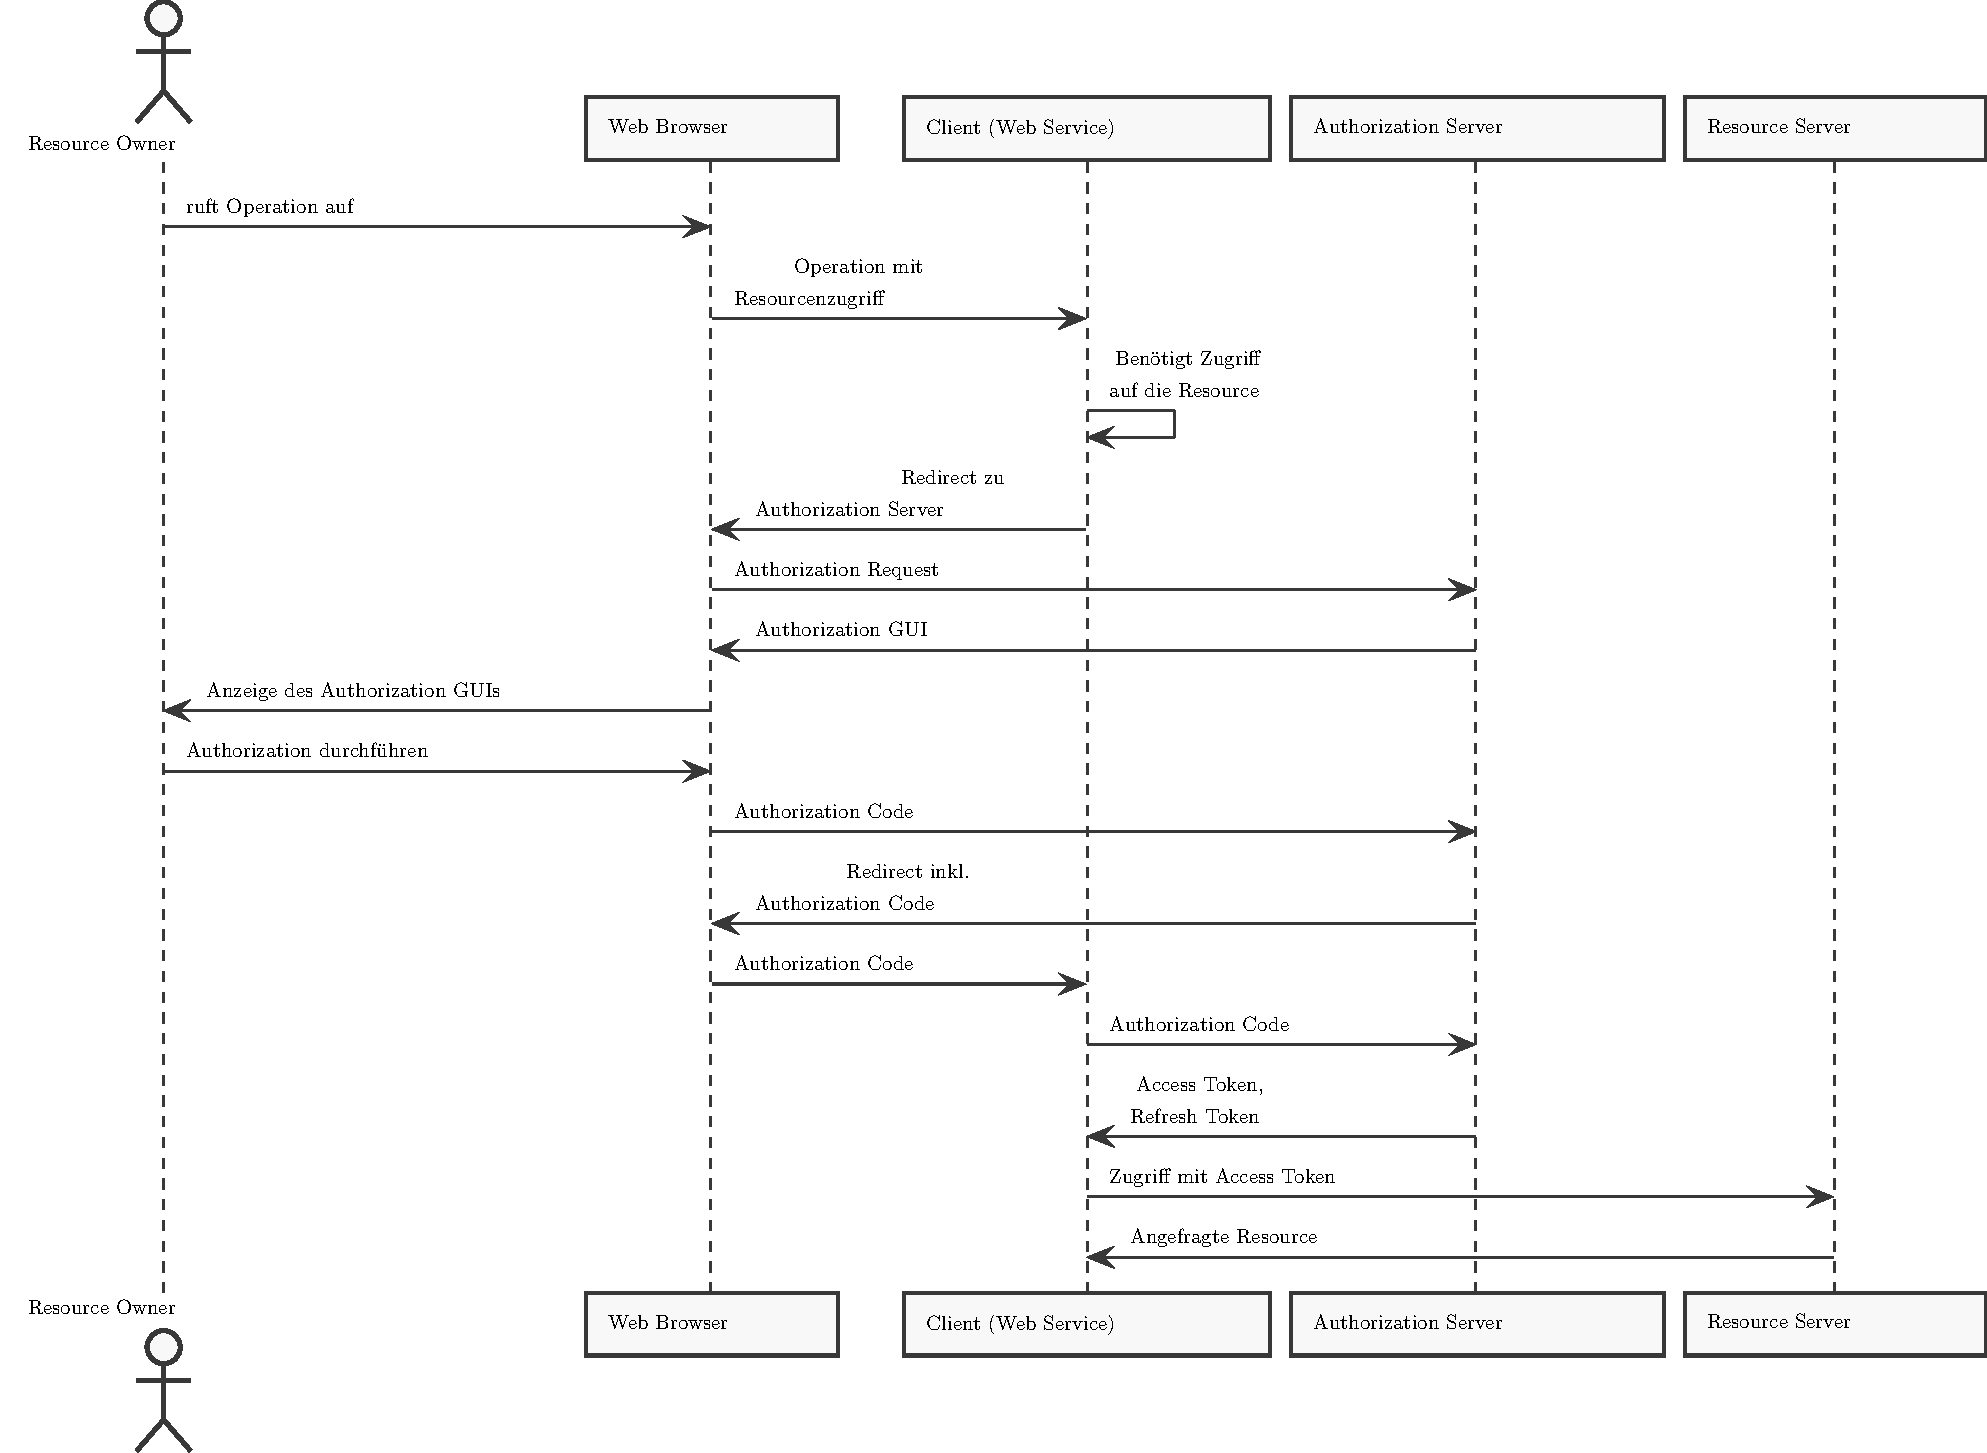
\includegraphics[width=\textwidth]{graphs/oauth2.pdf}
	\centering
\end{figure}

Ein interessanter Aspekt ist der Zeitpunkt der Authorization: die Überprüfung der eigentlich Zugriffsberechtigung wird durch den Authorization-Server zum Zeitpunkt der Ausstellung des Tokens durchgeführt. Bei einem Zugriff auf den Resourcen Server werden die eigentlichen Berechtigungen nicht mehr überprüft, sondern nur noch getestet ob das übergebene Token Zugriff auf die angeforderten Resourcen inkludiert und von einem validen Authorization Server signiert wurde.

Das Token besitzt eine Laufzeit und ist bis zum Ende der Laufzeit gültig. Da der Resource Server nicht direkt mit dem Authorization Server kommuniziert, gibt es keine Möglichkeit ein Token zuvorig zu invalidieren. Dies ist problematisch, falls eine lange Laufzeit (z. B. ein Jahr) gewählt wurde und ein Token abhanden gekommen ist. Ein Angreifer mit dem entwendeten Token kann nun bis zum Ende der Laufzeit dieses Token verwenden um auf die Resource zuzugreifen.

Um dieses Problem zu entschärfen werden zumeist zwei Tokens generiert: ein Access-Token und ein Refresh-Token. Das Access-Token wird zum Zugriff auf den Resource Server verwendet und besitzt eine sehr kurze Laufzeit, zumeist im Minuten-Bereich. Falls ein Access-Token abgelaufen ist, kann der Client das Refresh-Token verwenden um (ohne Benutzerinteraktion) ein neues Access-Token zu erhalten. Dies verbessert die Sicherheitssituation, da der Authorization-Server vor dem Ausstellen eines Access-Tokens überprüft, ob das Subject/der User überhaupt noch die notwendige Berechtigung besitzt. Dadurch wird das verwundbare Zeitfenster zwar nicht entfernt, aber zumindest reduziert.

\section{OpenID Connect}

OpenID-Connect verwendet OAuth2 um eine Benutzeridentifikation und -authentication umzusetzen.

\section{SAML2}

Die Abkürzung SAML2 steht für Security Assertion Markup Language (Version 2). Diese XML-basierte Sprache dient zum Austausch von Authentication und Authorization Informationen zwischen mehreren Parteien. Dabei will sich ein Benutzer mittels eines Clients (z. B. Webbrowser) an einem Service Provider (z. B. Webserver) anmelden. Um dies durchzuführen wird ein Identity Provider (IdP) bemühtdieser ist ein Service welches für einen User gegenüber einem Service Provider authentifiziert und authorized; ebenso kann dieser Serivce einen synchronen Single Sign-Out durchführen.

Die jeweiligen Operationen werden im SAML2 Jargon häufig \textit{Flows} genannt. Es gibt Login- und Logout-Flows, beide können entweder vom Service Provider oder vom Identity Provider gestartet werden. Diese unterschiedliche Ausprägung ist durch unterschiedliche Use-Cases bedingt. Falls ein Betrieb mehrere Websysteme betreibt, die eigenständig sind (z. B. eine GitLab-Instanz, eine NextCloud-Instanz), diese aber mit einem unified Sign-In versehen will, macht der SP-trigered flow Sinn. Der Benutzer wird beim Login auf z. B. GitLab zu dem IdP weitergeleitet und loggt sich auf diesem ein. Es wird eine Bestätigung für GitLab generiert (Token) und der User wird automatisch mit diesem Token zu dem GitLab-Server weitergeleitet (auf dem er nun eingeloggt ist). Den IdP-triggered flow würde man eher in einem Portal-Umfeld verwenden: hier gibt es eine initiale Login-Seite und dem Benutzer wird danach ein typisches Portal mit mehreren eigenständigen aber integrierten Applikationen angezeigt. Wenn er nun auf eine Subapplikation klickt, wird das Token automatisch mitübertragen und der User ist in der Subapplikation eingeloggt (ohne zuvorig vom SP zum IdP umgeleitet zu werden).

\subsection{SAML2 Assertions}

Das Herzstück von SAML2 sind die Security Assertions die vom IdP ausgestellt werden. Eine solche Assertion beschreibt die Rechte, welche ein User auf einem SP besitzt. Die Assertion wird vom IdP mittels einer public-key basierten Signatur unterschrieben.

Typische Elemente einer Assertion wären:

\begin{itemize}
	\item \textit{Issuer} identifiziert den IdP der diese Assertion ausgestellt hat.
	\item \textit{Signature} beinhaltet die Signatur welche die Integrität der Security Assertion sichert.
	\item \textit{Subject} beschreibt das identifizierte Objekt, in diesem Fall den identifizierten User. Der verwendete Identifier (\textit{NameId}) kann verschiedene Typen besitzen, häufig wird \textit{transient} verwendet. \textit{transient} beschreibt einen kurzfristigen Identifier, ähnlich einer Session-Id, und besitzt den Vorteil, dass auf diese Weise der SP nicht die genaue Identität des Subjects erfährt.
	\item Conditions: beliebig viele Conditions welche den Anwendungsbereich der Assertion beschränken. Beispiel sind z. b. temporale Beschränkungen (\textit{NotBefore}, \textit{NotOnOrAfter}) oder eine Einschränkung der Service für welche die Assertion gültig sein soll.
	\item AttributeStatement: beliebig viele Attribute-Statements welche optionale Daten an die Assertion anhängen.
	\item \textit{AuthnStatement} beschreibt die Assertion selbst und beinhaltet einen eindeutigen Identifier für die Assertion (\textit{SessionIndex}). Dieser Identifier wird häufig im Zuge des Sign-Out zur Identifikation der betroffenen Session verwendet.
\end{itemize}

Bei einem realen Deployment kann die Situation auftreten, dass mehrere Identity Provider verfügbar sind und der Service Provider den korrekten IdP selektieren muss. Ein Beispiel wäre ein Unternehmen welches interne User gegen einem Active Directory und externe User gegen einen öffentlichen IdP authentifiziert.

Um die Selektion des IdPs zu vereinfachen, gibt es das IdP Discovery Protokoll. Die beiden häufigen Arten des IdP Discoveries sind:

\begin{itemize}
	\item IdP Discovery am SP: der SP selbst kann die User einem IdP zuordnen und weis daher, welchen IdP er kontaktieren soll.
	\item Delegated IdP Discovery: der SP leitet die Anfrage an einen eigenen IdP Discovery Service weiter. Dieser identifiziert den zu wählenden IdP und retourniert diese Information an den SP. Bei diesem Protokoll muss erwähnt werden, dass die gesamte Kommunikation über den Client läuft: der SP teilt dem Client mit, dass dieser per HTTP Redirect den IdP Discovery Service kontaktieren soll (auf diese Weise erhält der IdP Discovery Service die IP des Clients).
\end{itemize}

\subsection{Protocol Bindings}

SAML2 dient zur Vereinheitlichung bestehender SSO-Lösung, daher wurde beim Entwurf des Standards auf vielfältige Integrationsmöglichkeiten in bestehende Netzwerke geachtet. Dementsprechend definiert SAML2 multiple Transportprotokolle, sogenannte Bindings:

\begin{itemize}
	\item HTTP Redirect Binding
	\item HTTP POST Binding
	\item HTTP Artifact Binding
	\item SAML SOAP Binding
	\item Reverse SOAP Binding
	\item SAML URI Binding
\end{itemize}

Bei Webbrowser-basierten Flows wird meistens das HTTP Redirect oder das HTTP POST Binding verwendet. Bei dem Redirect binding werden die übertragenen SAML Dokumente mittels Base64 codiert und als HTTP Parameter innerhalb von HTTP Redirects verwendet. Da die Länge der Parameter durch die jeweiligen Webbrowser limitiert ist, wird dieses Verfahren vor allem für kurze Nachrichten verwendet. HTTP POST basierte Verfahren verpacken die Nachrichten innerhalb von HTML Formularen und umgehen dadurch die Größenlimitierung. Um den Fluss zu automatisieren, werden die Formular zumeist mittels JavaScript automatisch versendet.

\subsection{Beispiel: Single Sign-On}

Hier ein Beispiel für ein SP-initiated Single-Sign on welches das HTTP POST Binding verwendet:

\begin{figure}[h!]
	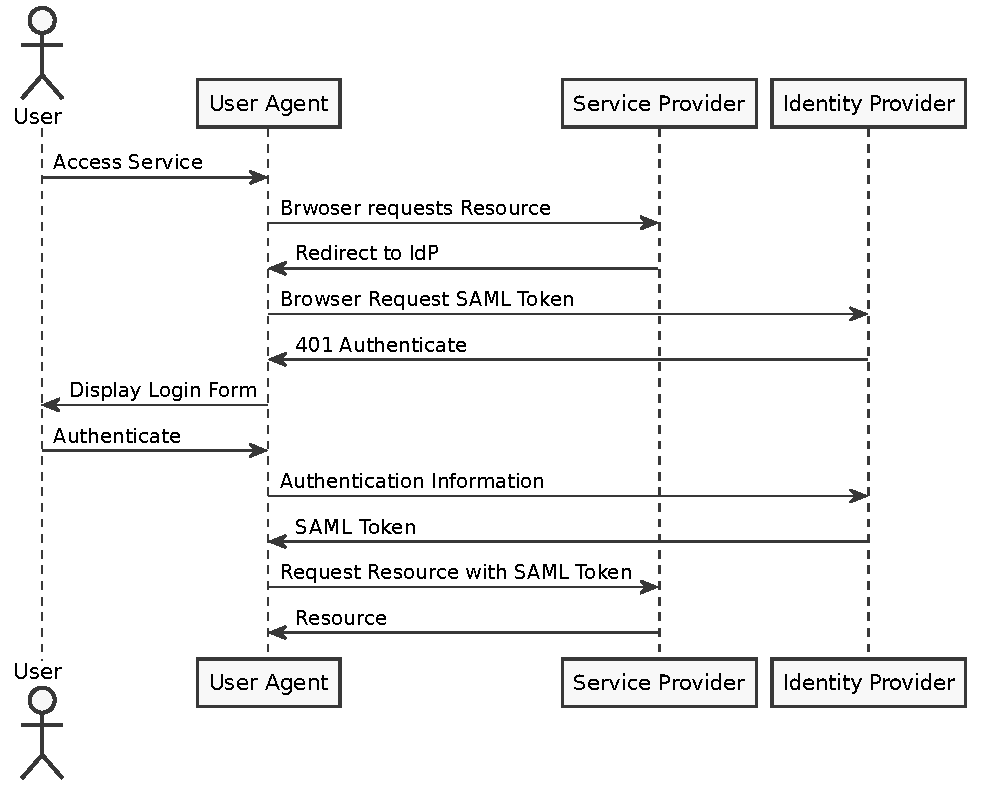
\includegraphics[width=\textwidth]{graphs/saml2.pdf}
	\centering
\end{figure}

In diesem Beispiel will ein Client (\textit{User Agent}) auf einen Service Provider zugreifen und benötigt hierfür eine Autorisierung. Nach dem initialen Client-Zugriff (Schritt 1) verwendet der SP zusammen mit dem Client das \textit{IdP Discovery} Protokoll um den zugehörigen IdP zu identifizieren. Sobald dieser bekannt ist, erstellt der SP einen Authorization Request und teilt diesen (samt der Adresse des IdPs) dem Client mit. Der Client kontaktiert nun den IdP und übermittelt den Request.

Der IdP authentiziert und authorized nun den Client. Falls dies erfolgreich durchgeführt wurde, wird eine SAML2 Security Assertion ausgestellt, vom IdP signiert und dem Client mitgeteilt. Da dies ein HTTP POST basierter Flow ist, erstellt der IdP ein HTML Formular, inkludiert in diesem HTML Formular das generierte SAML-Dokument (hidden field) und submitted das Formular automatisch mittels Javascript (Schritt 4). Der Client greift nun auf den SP zu und übermittelt die SAML assertion. Der SP verifiziert die Signatur und erstellt eine Session basierend auf den Daten innerhalb der Assertion. Bei Schritt 6 wird (wahrscheinlich, ist implementierungsabhängig) ein Session Cookie gesetzt, dass der Client bei allen weiteren Anfragen an den SP verwendet. Auf diese Weise sind nun alle folgenden Requests authentifiziert und authorisiert.

\section{Reflektionsfragen}

\begin{enumerate}
	\item Wie funktioniert der Sign-On Fluss bei SAML2?
	\item Wie funktioniert der Authorisierungsfluss bei OAuth2?
	\item Wie ist ein JSON Web Token aufgebaut? Welches Problem kann im Zusammenhang mit Verwechslungen der Signatur und er MAC-Adresse passieren?
	\item Welche Rolle übernimmt das IdP Discovery Protokoll innerhalb von SAML2?
	\item Gegeben eine SAML2 Example Assertion, was sagt diese aus (wer ist issuer? wer ist subject, etc.)?
\end{enumerate}
